%%
% Copyright (c) 2017 - 2022, Pascal Wagler;
% Copyright (c) 2014 - 2022, John MacFarlane
%
% All rights reserved.
%
% Redistribution and use in source and binary forms, with or without
% modification, are permitted provided that the following conditions
% are met:
%
% - Redistributions of source code must retain the above copyright
% notice, this list of conditions and the following disclaimer.
%
% - Redistributions in binary form must reproduce the above copyright
% notice, this list of conditions and the following disclaimer in the
% documentation and/or other materials provided with the distribution.
%
% - Neither the name of John MacFarlane nor the names of other
% contributors may be used to endorse or promote products derived
% from this software without specific prior written permission.
%
% THIS SOFTWARE IS PROVIDED BY THE COPYRIGHT HOLDERS AND CONTRIBUTORS
% "AS IS" AND ANY EXPRESS OR IMPLIED WARRANTIES, INCLUDING, BUT NOT
% LIMITED TO, THE IMPLIED WARRANTIES OF MERCHANTABILITY AND FITNESS
% FOR A PARTICULAR PURPOSE ARE DISCLAIMED. IN NO EVENT SHALL THE
% COPYRIGHT OWNER OR CONTRIBUTORS BE LIABLE FOR ANY DIRECT, INDIRECT,
% INCIDENTAL, SPECIAL, EXEMPLARY, OR CONSEQUENTIAL DAMAGES (INCLUDING,
% BUT NOT LIMITED TO, PROCUREMENT OF SUBSTITUTE GOODS OR SERVICES;
% LOSS OF USE, DATA, OR PROFITS; OR BUSINESS INTERRUPTION) HOWEVER
% CAUSED AND ON ANY THEORY OF LIABILITY, WHETHER IN CONTRACT, STRICT
% LIABILITY, OR TORT (INCLUDING NEGLIGENCE OR OTHERWISE) ARISING IN
% ANY WAY OUT OF THE USE OF THIS SOFTWARE, EVEN IF ADVISED OF THE
% POSSIBILITY OF SUCH DAMAGE.
%%

%%
% This is the Eisvogel pandoc LaTeX template.
%
% For usage information and examples visit the official GitHub page:
% https://github.com/Wandmalfarbe/pandoc-latex-template
%%

% Options for packages loaded elsewhere
\PassOptionsToPackage{unicode}{hyperref}
\PassOptionsToPackage{hyphens}{url}
\PassOptionsToPackage{dvipsnames,svgnames,x11names,table}{xcolor}
%
\documentclass[
  paper=a4,
  ,captions=tableheading
]{scrartcl}
\usepackage{amsmath,amssymb}
% Use setspace anyway because we change the default line spacing.
% The spacing is changed early to affect the titlepage and the TOC.
\usepackage{setspace}
\setstretch{1.2}
\usepackage{iftex}
\ifPDFTeX
  \usepackage[T1]{fontenc}
  \usepackage[utf8]{inputenc}
  \usepackage{textcomp} % provide euro and other symbols
\else % if luatex or xetex
  \usepackage{unicode-math} % this also loads fontspec
  \defaultfontfeatures{Scale=MatchLowercase}
  \defaultfontfeatures[\rmfamily]{Ligatures=TeX,Scale=1}
\fi
\usepackage{lmodern}
\ifPDFTeX\else
  % xetex/luatex font selection
\fi
% Use upquote if available, for straight quotes in verbatim environments
\IfFileExists{upquote.sty}{\usepackage{upquote}}{}
\IfFileExists{microtype.sty}{% use microtype if available
  \usepackage[]{microtype}
  \UseMicrotypeSet[protrusion]{basicmath} % disable protrusion for tt fonts
}{}
\makeatletter
\@ifundefined{KOMAClassName}{% if non-KOMA class
  \IfFileExists{parskip.sty}{%
    \usepackage{parskip}
  }{% else
    \setlength{\parindent}{0pt}
    \setlength{\parskip}{6pt plus 2pt minus 1pt}}
}{% if KOMA class
  \KOMAoptions{parskip=half}}
\makeatother
\usepackage{xcolor}
\definecolor{default-linkcolor}{HTML}{A50000}
\definecolor{default-filecolor}{HTML}{A50000}
\definecolor{default-citecolor}{HTML}{4077C0}
\definecolor{default-urlcolor}{HTML}{4077C0}
\usepackage[margin=2.5cm,includehead=true,includefoot=true,centering,]{geometry}
% add backlinks to footnote references, cf. https://tex.stackexchange.com/questions/302266/make-footnote-clickable-both-ways
\usepackage{footnotebackref}
\usepackage{graphicx}
\makeatletter
\def\maxwidth{\ifdim\Gin@nat@width>\linewidth\linewidth\else\Gin@nat@width\fi}
\def\maxheight{\ifdim\Gin@nat@height>\textheight\textheight\else\Gin@nat@height\fi}
\makeatother
% Scale images if necessary, so that they will not overflow the page
% margins by default, and it is still possible to overwrite the defaults
% using explicit options in \includegraphics[width, height, ...]{}
\setkeys{Gin}{width=\maxwidth,height=\maxheight,keepaspectratio}
% Set default figure placement to htbp
\makeatletter
\def\fps@figure{htbp}
\makeatother
\setlength{\emergencystretch}{3em} % prevent overfull lines
\providecommand{\tightlist}{%
  \setlength{\itemsep}{0pt}\setlength{\parskip}{0pt}}
\setcounter{secnumdepth}{5}
\usepackage{float}
\usepackage{booktabs}
\usepackage{longtable}
\usepackage{array}
\usepackage{multirow}
\usepackage{wrapfig}
\usepackage{colortbl}
\usepackage{pdflscape}
\usepackage{tabu}
\usepackage{threeparttable}
\usepackage{threeparttablex}
\usepackage[normalem]{ulem}
\usepackage{makecell}
\usepackage{xcolor}
\ifLuaTeX
  \usepackage{selnolig}  % disable illegal ligatures
\fi
\IfFileExists{bookmark.sty}{\usepackage{bookmark}}{\usepackage{hyperref}}
\IfFileExists{xurl.sty}{\usepackage{xurl}}{} % add URL line breaks if available
\urlstyle{same}
\hypersetup{
  pdftitle={Diamonds: Predictive Analysis of Price},
  pdfauthor={Francisco Arrieta, Emily Schmidt and Lucia Camenisch},
  hidelinks,
  breaklinks=true,
  pdfcreator={LaTeX via pandoc with the Eisvogel template}}
\title{Diamonds: Predictive Analysis of Price}
\author{Francisco Arrieta, Emily Schmidt and Lucia Camenisch}
\date{21 December 2022}



%%
%% added
%%


%
% for the background color of the title page
%
\usepackage{pagecolor}
\usepackage{afterpage}
\usepackage{tikz}
\usepackage[margin=2.5cm,includehead=true,includefoot=true,centering]{geometry}

%
% break urls
%
\PassOptionsToPackage{hyphens}{url}

%
% When using babel or polyglossia with biblatex, loading csquotes is recommended
% to ensure that quoted texts are typeset according to the rules of your main language.
%
\usepackage{csquotes}

%
% captions
%
\definecolor{caption-color}{HTML}{777777}
\usepackage[font={stretch=1.2}, textfont={color=caption-color}, position=top, skip=4mm, labelfont=bf, singlelinecheck=false, justification=raggedright]{caption}
\setcapindent{0em}

%
% blockquote
%
\definecolor{blockquote-border}{RGB}{221,221,221}
\definecolor{blockquote-text}{RGB}{119,119,119}
\usepackage{mdframed}
\newmdenv[rightline=false,bottomline=false,topline=false,linewidth=3pt,linecolor=blockquote-border,skipabove=\parskip]{customblockquote}
\renewenvironment{quote}{\begin{customblockquote}\list{}{\rightmargin=0em\leftmargin=0em}%
\item\relax\color{blockquote-text}\ignorespaces}{\unskip\unskip\endlist\end{customblockquote}}

%
% Source Sans Pro as the de­fault font fam­ily
% Source Code Pro for monospace text
%
% 'default' option sets the default
% font family to Source Sans Pro, not \sfdefault.
%
\ifnum 0\ifxetex 1\fi\ifluatex 1\fi=0 % if pdftex
    \usepackage[default]{sourcesanspro}
  \usepackage{sourcecodepro}
  \else % if not pdftex
    \usepackage[default]{sourcesanspro}
  \usepackage{sourcecodepro}

  % XeLaTeX specific adjustments for straight quotes: https://tex.stackexchange.com/a/354887
  % This issue is already fixed (see https://github.com/silkeh/latex-sourcecodepro/pull/5) but the
  % fix is still unreleased.
  % TODO: Remove this workaround when the new version of sourcecodepro is released on CTAN.
  \ifxetex
    \makeatletter
    \defaultfontfeatures[\ttfamily]
      { Numbers   = \sourcecodepro@figurestyle,
        Scale     = \SourceCodePro@scale,
        Extension = .otf }
    \setmonofont
      [ UprightFont    = *-\sourcecodepro@regstyle,
        ItalicFont     = *-\sourcecodepro@regstyle It,
        BoldFont       = *-\sourcecodepro@boldstyle,
        BoldItalicFont = *-\sourcecodepro@boldstyle It ]
      {SourceCodePro}
    \makeatother
  \fi
  \fi

%
% heading color
%
\definecolor{heading-color}{RGB}{40,40,40}
\addtokomafont{section}{\color{heading-color}}
% When using the classes report, scrreprt, book,
% scrbook or memoir, uncomment the following line.
%\addtokomafont{chapter}{\color{heading-color}}

%
% variables for title, author and date
%
\usepackage{titling}
\title{Diamonds: Predictive Analysis of Price}
\author{Francisco Arrieta, Emily Schmidt and Lucia Camenisch}
\date{21 December 2022}

%
% tables
%

%
% remove paragraph indention
%
\setlength{\parindent}{0pt}
\setlength{\parskip}{6pt plus 2pt minus 1pt}
\setlength{\emergencystretch}{3em}  % prevent overfull lines

%
%
% Listings
%
%


%
% header and footer
%
\usepackage[headsepline,footsepline]{scrlayer-scrpage}

\newpairofpagestyles{eisvogel-header-footer}{
  \clearpairofpagestyles
  \ihead*{Diamonds: Predictive Analysis of Price}
  \chead*{}
  \ohead*{21 December 2022}
  \ifoot*{Francisco Arrieta, Emily Schmidt and Lucia Camenisch}
  \cfoot*{}
  \ofoot*{\thepage}
  \addtokomafont{pageheadfoot}{\upshape}
}
\pagestyle{eisvogel-header-footer}



%%
%% end added
%%

%% adding more size options for the title
\usepackage{moresize}

%% other tabulars
\usepackage{tabu}

\begin{document}

%%
%% begin titlepage
%%
\begin{titlepage}
\newgeometry{top=2cm, right=4cm, bottom=3cm, left=4cm}
\tikz[remember picture,overlay] \node[inner sep=0pt] at (current page.center){
\includegraphics[width=\paperwidth,height=\paperheight]{diamond-background.jpeg}};
\newcommand{\colorRule}[3][black]{\textcolor[HTML]{#1}{\rule{#2}{#3}}}
\begin{flushleft}
\noindent
\\[-1em]
\color[HTML]{D8B365}
\makebox[0pt][l]{\colorRule[D8B365]{1.3\textwidth}{4pt}}
\par
\noindent

% The titlepage with a background image has other text spacing and text size
{
  \setstretch{2}
  \vfill
  \vskip -8em
  \noindent {\HUGE \textbf{\textsf{Diamonds: Predictive Analysis of
Price}}}
    \vskip 2em
  \noindent {\Large \textsf{Francisco Arrieta, Emily Schmidt and Lucia
Camenisch} \vskip 0.6em \textsf{21 December 2022}}
  \vfill
}


\end{flushleft}
\end{titlepage}
\restoregeometry
\pagenumbering{arabic}

%%
%% end titlepage
%%

% \maketitle


{
\setcounter{tocdepth}{4}
\tableofcontents
}
\hypertarget{introduction}{%
\section{Introduction}\label{introduction}}

The following report provides the result of using machine learning as a
tool to estimate diamond prices for a jewelry company. Using snapshot
information from their asset database, various methods were applied to
train predictive models using regression analysis. The main objective
was to use supervised learning methods to predict prices. These models
are later compared to measure their effectiveness by using error
measurements to quantify the distance between the prediction and the
actual price. Finally, conclusions on the capability of each model are
made and suggestions are given on which model to apply for the problem
at hand.

The product being analyzed is diamonds. Being a luxury object with a
long history, industry standards have been developed to serve as
guidelines for estimating the value of the product. A wide variety of
characteristics affect the overall price of diamonds, but this analysis
will focus on their physical qualities, such as size dimensions, size
ratios and color. Other factors inherent to scarce products in high
demand of a capitalist economy will not be considered in our machine
learning exercise.

The choice of methods shown in the report is not all inclusive and
responds to the fact of only being some of the most used methods to this
day. By implementing them, the analysts hope to provide a glimpse of the
effects and importance in choosing the right model as well as displaying
the differences between each one.

\hypertarget{data-exploration}{%
\section{Data Exploration}\label{data-exploration}}

In the early stages of any analysis, data exploration is a critical
process aimed at understanding and analyzing the data set to gain
insight and make valid decisions. The overarching goal of examining the
data is to obtain intuition, identify questionable values, and
strategize how to answer the problem statement. Therefore, let's
summarize the findings that explain the main data characteristics, and
dive into the relations between variables.

\hypertarget{dimension-summary}{%
\subsection{Dimension Summary}\label{dimension-summary}}

There is a variety of ways an analyst could approach understanding the
observations in the data set. For starters, there are 53,940 records and
10 variables.

\begin{itemize}
\item
  \texttt{price}: The response variable which is measured in USD and
  ranges between \$326 to \$18,823
\item
  \texttt{carat}: Continuous value that gives information about the
  weight of the diamond (1 ct = 200 mg)
\item
  \texttt{cut}: Quality of the circular cut and has five levels (worst:
  \texttt{Fair} \textbar{} best: \texttt{Ideal})
\item
  \texttt{color}: The less color within the diamond the better
  (yellow-ish: \texttt{J} \textbar{} clear: \texttt{D})
\item
  \texttt{clarity}: A categorical value that measures how clear the
  diamond appears without impurities (worst: \texttt{I1} \textbar{}
  best: \texttt{IF})
\item
  \texttt{x}: A numeric variable that relates to the diamond
  \texttt{length} in millimeters (mm), which ranges from 0.00 mm to
  10.74 mm
\item
  \texttt{y}: A numeric variable that relates to the diamond
  \texttt{width} in millimeters (mm), which ranges from 0 mm to 58.90 mm
\item
  \texttt{z}: A numeric variable that relates to the diamond
  \texttt{depth}/height in millimeters (mm), which ranges from 0 mm to
  31.80 mm
\item
  \texttt{depth\ total}: A calculated value that is computed with
  \texttt{x}, \texttt{y}, and \texttt{z} in terms of a percentage. This
  feature does not exceed 79.00\%
\item
  \texttt{table}: The width of the top of diamond relative to widest
  point that can be seen when the stone is viewed face up
\end{itemize}

The outcome variable (\texttt{price}) is a an integer. There are an
additional six numeric values and three ordinal/categorical features
that have a factored structure. Those non-numeric values (\texttt{cut},
\texttt{color}, and \texttt{clarity}) need to be appropriately ordered,
and renamed if there are any spaces within their naming convention as
later this could obstruct certain code.

\begin{figure}[H]

{\centering 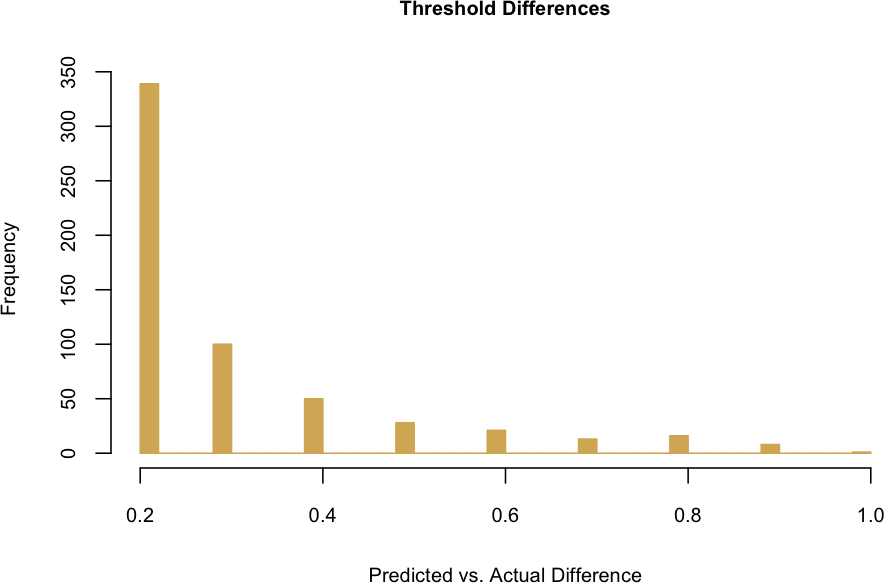
\includegraphics[width=0.5\linewidth,]{Diamonds_PDF_files/figure-latex/threshold diff hist-1}

}

\caption{Amount of records by difference between computed depth ratio and actual depth ratio}\label{fig:threshold diff hist}
\end{figure}

To dive deeper, we consider removing records that are invalid because
they add noise. For instance, price against all features were reviewed
for possible impurities. In total, there are 275 (0.5\%) rows removed
for the following reasons:

\begin{enumerate}
\def\labelenumi{\arabic{enumi}.}
\item
  20 rows had a depth of 0.00. This was considered inaccurate because a
  diamond needs to have this dimension specified.
\item
  The difference between length and width should be almost identical
  since the diamond should be cut approximately circular. If they were
  not, those rows were removed. In this case, only two records were not
  included in the data set at differences above 36.00 mm.
\item
  The depth\_ratio is a calculation between \texttt{length}
  (\texttt{x}), \texttt{width} (\texttt{y}), and \texttt{depth}
  (\texttt{z}). To investigate this feature further, our group computed
  \texttt{depth\_ratio} and saw there were differences between the
  actual and predicted values. As seen in \textbf{Figure 1}, most errors
  were at 0.2, hence the executive decision was to remove any
  differences above a threshold of 0.3. A total of 253 rows were
  removed.
\end{enumerate}

In the remaining 53,918 observations, there were no missing values.

In continuation of exploring the diamonds dataset, we now look at the
relationships between variables. By isolating price against the other
continuous variables, it is seen that \texttt{carat}, \texttt{length},
\texttt{width}, and \texttt{depth}, all have a positively linear
relation to the response feature. Some of the models used in the
analysis to predict price will show these effects later as a possible
issue of collinearity could occur. In addition, the relationship between
carat and price is unique because their relation is non-linear. We were
also interested in showing how the categorical variables affect price.
\texttt{clarity}, \texttt{color}, and \texttt{cut} have distinct
patterns seen between the four continuous variables mentioned above.

\begin{figure}[H]

{\centering 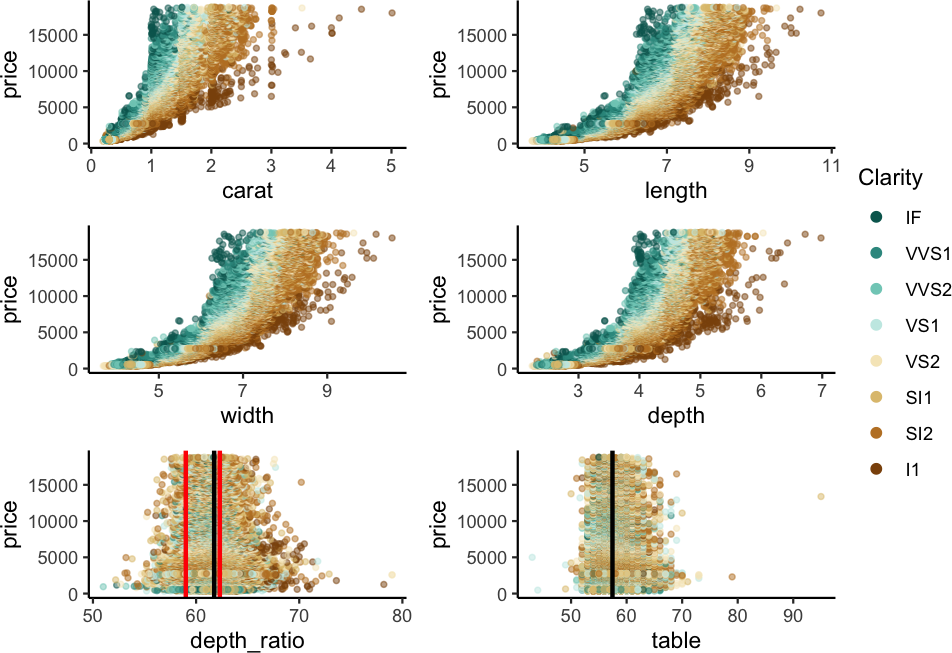
\includegraphics[width=\linewidth,]{Diamonds_PDF_files/figure-latex/Price by X and Clarity-1}

}

\caption{Price with respect to numerical variables, by Clarity}\label{fig:Price by X and Clarity}
\end{figure}

When plotting \texttt{price} by \texttt{carat}, \texttt{width},
\texttt{length}, and \texttt{depth}, with \texttt{clarity} as the color
dimension, there is a clear distinction between how these observations
relate. Each scatter plot shows a strong, positive correlation to
\texttt{price}. When reviewing the x-axis for each explanatory variable,
the lower tiered option is typically observed more. The cheaper the
gemstone, the worse quality. Within each plot, there are outliers that
can be explained by how the diamond was cut, which impacts the
\texttt{weight}, \texttt{length}, and \texttt{depth}. By the color
scale, it is noticed how there are more diamonds with a worse clarity
(SI2/SI1) than there are with the best (IF/VVS1). Intuitively, this
makes sense because perfecting a diamond's clarity is quite difficult.
Therefore, a majority of the diamonds lie between the second and third
best, and second and third worst clarity factors. In addition, the
relation between \texttt{depth\_ratio} and \texttt{table} to
\texttt{price} is not distinct as those features are mixed throughout
the relative ranges. Within all of the \texttt{depth\_ratio} plots,
there are vertical lines that show the \texttt{depth\_ratio} mean
(black) and range (red) of what is considered the prime value for
\texttt{depth\_ratio} as long as it is above 59.00\% but does not exceed
62.30\%.

\begin{figure}[H]

{\centering 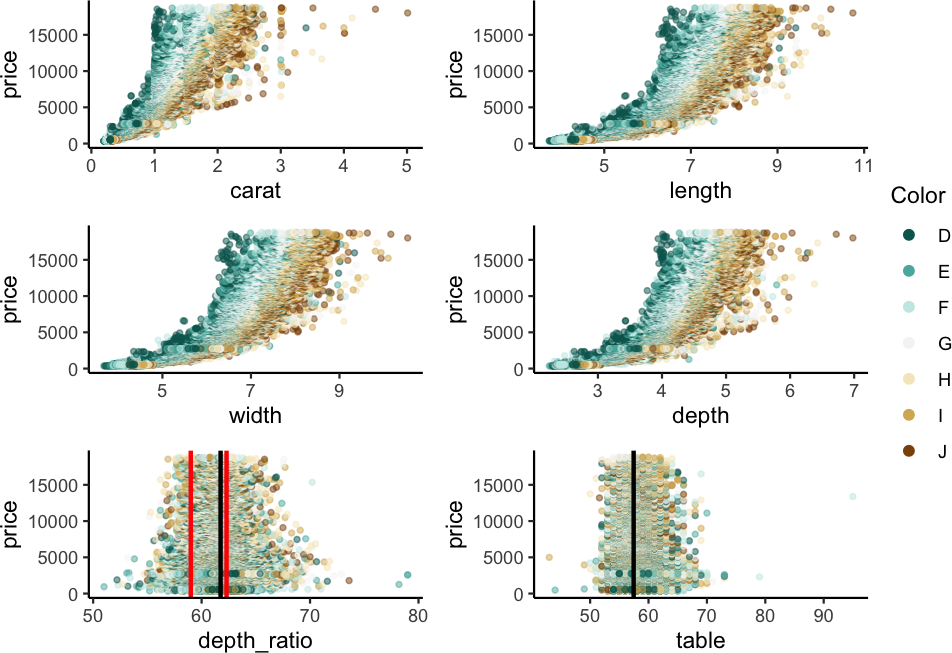
\includegraphics[width=\linewidth,]{Diamonds_PDF_files/figure-latex/Price by X and Color-1}

}

\caption{Price with respect to numerical variables, by Color}\label{fig:Price by X and Color}
\end{figure}

A similar relationship can be seen regarding \texttt{price} by the
continuous variables, but as \texttt{color} as the color dimension.
Instead of a majority the observations falling closer to the best and
worst \texttt{clarity} features, here the reader will notice how it
appears that the colors E, F and G dominate (the white to light blue)
the space.

\begin{figure}[H]

{\centering 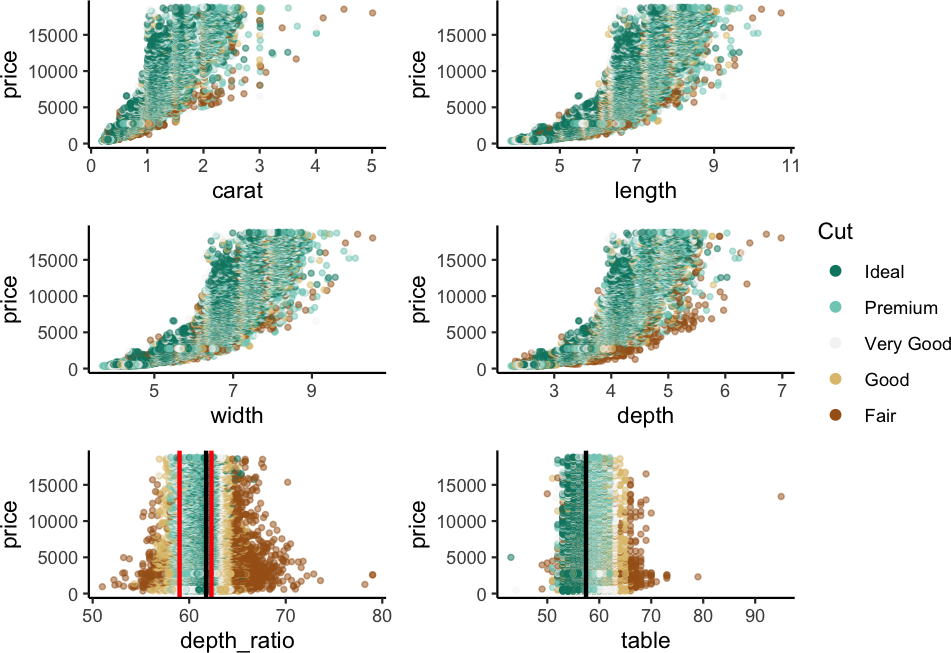
\includegraphics[width=\linewidth,]{Diamonds_PDF_files/figure-latex/Price by X and Cut-1}

}

\caption{Price with respect to numerical variables, by Cut}\label{fig:Price by X and Cut}
\end{figure}

\texttt{Cut} has completely different trends than \texttt{clarity} and
\texttt{color} as a majority of the diamonds are either \texttt{Ideal}
or \texttt{Premium}. This can especially be seen within the
\texttt{depth\_ratio} plot. As stated earlier, the red lines indicate
the optimal space in which the luxury brand attempts to get the best
ratio. Most of all of the prime cuts are within those bounds while the
\texttt{Fair}, \texttt{Good}, and \texttt{Very\ good} are outside. There
is a clear distinction on how \texttt{cut} relates to the
\texttt{depth\_ratio} along \texttt{price}.

\hypertarget{variable-visualisation}{%
\subsection{Variable Visualisation}\label{variable-visualisation}}

This section involves creating graphical representations of data to
visually communicate insights and trends. It allows us to quickly and
easily identify patterns that may not be immediately apparent from
looking at raw data. There are several graphics that demonstrate how
these qualitative and quantitative variables are distributed. Since some
models take into account transformation, those details will be described
later.

\begin{figure}[H]

{\centering 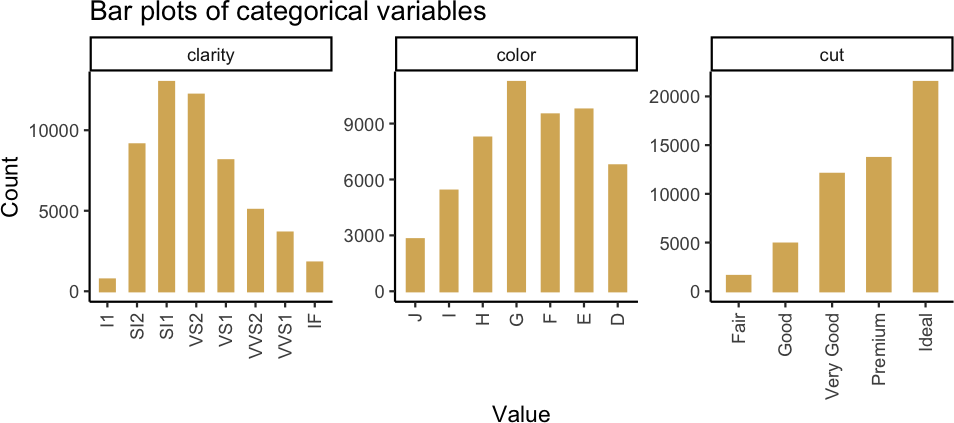
\includegraphics[width=\linewidth,]{Diamonds_PDF_files/figure-latex/categorical bar plots-1}

}

\caption{Bar plots of categorical variables}\label{fig:categorical bar plots}
\end{figure}

Recall the variable descriptions in the beginning of the exploratory
data analysis.

\begin{itemize}
\item
  \texttt{clarity}: After the worst clarity (\texttt{I1}), the bulk of
  diamonds range from \texttt{SI2} and \texttt{VS1}. This correlates to
  the scatter plot with the goldish toned points as there appear to be
  more of those diamonds than ones with better clarity.
\item
  \texttt{cut}: The less yellow the diamond, the better. The dataset
  shows that most diamonds are either \texttt{G}, \texttt{F}, or
  \texttt{E}, which are the closest three to the least colored diamond.
\item
  \texttt{color}: There are over 20,000 diamonds that have an
  \texttt{ideal} cut which \texttt{premium} and \texttt{very\ good}
  between 10,000 and 15,000.
\end{itemize}

\begin{figure}[H]

{\centering 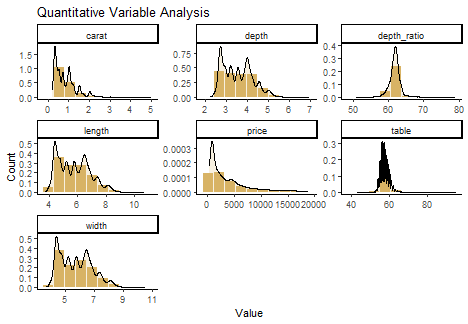
\includegraphics[width=\linewidth,]{Diamonds_PDF_files/figure-latex/Histograms-1}

}

\caption{Histograms of numerical variables}\label{fig:Histograms}
\end{figure}

\begin{figure}[H]

{\centering 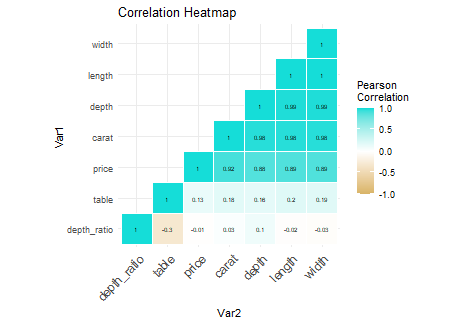
\includegraphics[width=0.5\linewidth,]{Diamonds_PDF_files/figure-latex/Correlation-1}

}

\caption{Correlation heatmap of numerical variables}\label{fig:Correlation}
\end{figure}

At a high-level, \texttt{price} and \texttt{carat} can be seen as
positively skewed. In the scatter plot regarding \texttt{price} by
\texttt{cut} for the \texttt{depth\_ratio}, the histogram also displays
the same conclusion that the cut features fall into approximately 60 to
65 mm. The relationships in the Correlation Heat Map visually show how
\texttt{width}, \texttt{length}, \texttt{depth}, and \texttt{carat}
continue to be highly correlated with \texttt{price} while
\texttt{depth\_ratio} and \texttt{table} are closer to 0.

Through exploration, we can gain a deeper understanding of the data and
how it can be used to answer business questions or solve real-world
problems, like predicting the price of a diamond.

\hypertarget{variable-prediction-and-model-performance-evaluation}{%
\section{Variable Prediction and Model Performance
Evaluation}\label{variable-prediction-and-model-performance-evaluation}}

\hypertarget{linear-regression}{%
\subsection{Linear Regression}\label{linear-regression}}

\hypertarget{data-preparation}{%
\subsubsection{Data preparation}\label{data-preparation}}

We begin by performing linear regressions on our data. As we saw during
the exploration phase, some predictors (\texttt{carat}, \texttt{length},
\texttt{width} and \texttt{depth}) are highly correlated. Therefore,
multicollinearity might be an issue.

We use the Generalized Variation Inflation Factors (GVIF) to measure the
multicollinearity level of our data. This generalized version of the VIF
allows us to take into account numerical and categorical predictors
together. The GVIF clearly confirms that there is an issue, as
\texttt{length}, \texttt{width} and \texttt{depth} all have coefficients
above 1000. \texttt{carat} and \texttt{depth\_ratio} also have high
values above 25, but they aren't as high extreme as the other three.

After removing \texttt{length}, \texttt{width} and \texttt{depth}, the
GVIF coefficients of the remaining predictors are all under 2, which
indicates the multicollinearity problem is solved. We display
correlation ellipses of numerical variables.

\begin{figure}[H]

{\centering 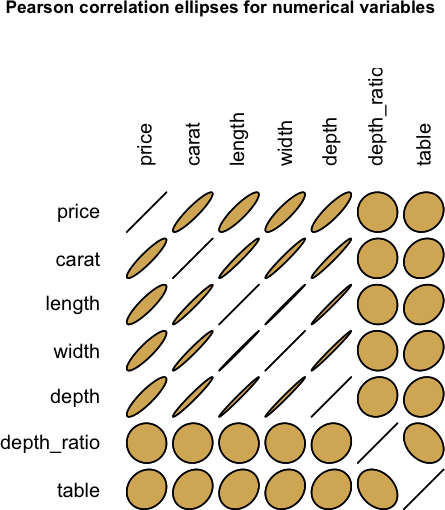
\includegraphics[width=0.4\linewidth,]{Diamonds_PDF_files/figure-latex/uncorrelated-ellipses-1}

}

\caption{Correlation ellipses for numerical variables}\label{fig:uncorrelated-ellipses}
\end{figure}

Thus, we will perform linear regressions on two different models:

\begin{enumerate}
\def\labelenumi{\arabic{enumi}.}
\tightlist
\item
  \texttt{LM\_complete} which contains all predictors
\item
  \texttt{LM\_minus\_corr} which has \texttt{length}, \texttt{width} and
  \texttt{depth} removed.
\end{enumerate}

These two models will serve as basis for variable selection procedures
later.

However, before starting to build our models, we also need to account
for skewed variables. Linear regression might perform worse when dealing
with skewed variables and it is common to use transformations such as a
logarithm or a \(n\)th root to make variables more symmetrical.

We use an estimator of skewness called \(b_1\), whose definition can be
found
\href{https://en.wikipedia.org/wiki/Skewness\#Sample_skewness}{here}.

The value of \(b_1\) is interpreted as follows:

\begin{itemize}
\tightlist
\item
  \(0 \leq |b_1| < 0.5\): variable is symmetrical;
\item
  \(0.5 \leq |b_1| < 1\): variable is moderately skewed;
\item
  \(|b_1| \geq 1\): variable is highly skewed.
\end{itemize}

We compute \(b_1\) on our numerical variables and get the following
results.

\begin{table}[!h]

\caption{\label{tab:skewness-table}Skewness estimator for numerical variables}
\centering
\begin{tabu} to \linewidth {>{\raggedright}X>{\raggedleft}X}
\hline
  & b\_1\\
\hline
price & 1.6259747\\
\hline
carat & 1.0967514\\
\hline
length & 0.3984689\\
\hline
width & 0.3922008\\
\hline
depth & 0.3921093\\
\hline
depth\_ratio & 0.0182498\\
\hline
table & 0.8728869\\
\hline
\end{tabu}
\end{table}

\texttt{price} and \texttt{carat} are highly skewed and \texttt{table}
is moderately skewed.

We apply a logarithmic transformation to all three variables. The
improvement can also be seen in the histograms, as they look more
symmetrical now.

\begin{figure}[H]

{\centering 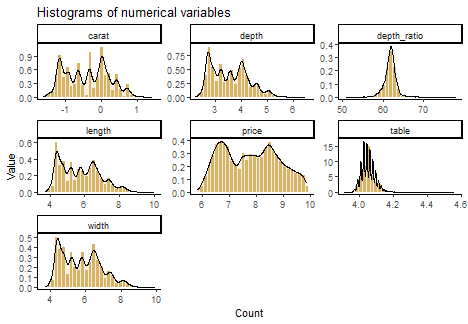
\includegraphics[width=\linewidth,]{Diamonds_PDF_files/figure-latex/hist-unskewed-1}

}

\caption{Histograms of numerical variables after unskewing}\label{fig:hist-unskewed}
\end{figure}

We also standardize numerical variables by subtracting their mean and
dividing by their standard deviation. This makes the comparison of
\(\beta\) coefficients between variables easier.

\hypertarget{linear-models}{%
\subsubsection{Linear models}\label{linear-models}}

The data is now ready for our linear models. For both
\texttt{LM\_complete} and \texttt{LM\_minus\_corr}, we perform the
following linear regressions:

\begin{enumerate}
\def\labelenumi{\arabic{enumi}.}
\tightlist
\item
  Linear regression on the whole model
\item
  Forward selection on the model (iterative method)
\item
  Backward selection on the model (iterative method)
\item
  Stepwise selection on the model (iterative method)
\item
  Mallows's \(C_p\) and AIC selection on the model (global method)
\end{enumerate}

\hypertarget{summary-of-models}{%
\subsubsection{Summary of models}\label{summary-of-models}}

For each of these models, we summarise which variables are used as
predictors in the following table.

\begin{table}[!h]

\caption{\label{tab:Variable Selection Summary}Predictors used in each linear model}
\centering
\resizebox{\linewidth}{!}{
\begin{tabular}[t]{l c c c c c c c c c}
\hline
Model & Cut & Color & Clarity & Carat & Length & Width & Depth & Depth Ratio & Table\\
\hline
LM\_complete & X & X & X & X & X & X & X & X & X\\
\hline
LM\_forward\_complete & X & X & X & X & X & X & X & X & X\\
\hline
LM\_backward\_complete & X & X & X & X & X &  & X & X & \\
\hline
LM\_stepwise\_complete & X & X & X & X & X &  & X & X & \\
\hline
LM\_CpAIC\_complete & X & X & X & X & X &  & X & X & \\
\hline
LM\_minus\_corr & X & X & X & X &  &  &  & X & X\\
\hline
LM\_forward\_minus\_corr & X & X & X & X &  &  &  & X & X\\
\hline
LM\_backward\_minus\_corr & X & X & X & X &  &  &  & X & \\
\hline
LM\_stepwise\_minus\_corr & X & X & X & X &  &  &  & X & \\
\hline
LM\_CpAIC\_minus\_corr & X & X & X & X &  &  &  & X & \\
\hline
\end{tabular}}
\end{table}

For both basis models, forward selection doesn't discard any variables,
whereas backward, stepwise and global selections all choose the same
model with less variables than initially.

Thus, we have four distinct models in total. We assess the predictive
performance of these four models on our validation set by computing the
five accuracy measures seen during the course.

Let us recall the definitions and meaning of the two main measures we
will use (taken from Data Mining for Business Analytics - Concepts,
Techniques, and Applications in R, chapter 5.2, page 119). We denote the
residuals by \(r = y - \hat y\).

\begin{enumerate}
\def\labelenumi{\arabic{enumi}.}
\tightlist
\item
  \textbf{ME} (Mean Error) gives an indication of whether the
  predictions are on average over- or under-predicting the outcome
  variable. \[ME = \dfrac{1}{n} \sum_{i=1}^{n}r_i\]
\item
  \textbf{RMSE} (Root Mean Squared Error) is similar to the standard
  error of estimate in linear regression, except that it is computed on
  the validation data rather than on the training data.
  \[RMSE =  \sqrt{\dfrac{1}{n}\sum_{i=1}^{n}r_i^2}\]
\end{enumerate}

\hypertarget{accuracy-measures-of-models-on-validation-set}{%
\subsubsection{Accuracy measures of models on validation
set}\label{accuracy-measures-of-models-on-validation-set}}

The accuracy measures for our four models are summarized below. In order
to give meaningful results, the outcome variable \texttt{price} has been
rescaled to its original scale and retransformed by taking the
exponential (to cancel out the logarithm). Thus, the ME, RMSE and MAE
can be interpreted in the price currency, dollars.

\begin{table}[!h]

\caption{\label{tab:models-accuracy-table}Accuracy measures of linear models}
\centering
\resizebox{\linewidth}{!}{
\begin{tabular}[t]{l r r r r r}
\hline
Model & ME & RMSE & MAE & MPE & MAPE\\
\hline
LM\_complete & 36.36648 & 846.5888 & 408.5364 & -0.8377036 & 10.33643\\
\hline
LM\_CpAIC\_complete & 36.32774 & 845.5018 & 408.1349 & -0.8408540 & 10.33659\\
\hline
LM\_minus\_corr & 50.38994 & 810.1522 & 405.0486 & -0.8420621 & 10.39559\\
\hline
LM\_CpAIC\_minus\_corr & 50.39878 & 810.1610 & 405.0616 & -0.8418121 & 10.39568\\
\hline
\end{tabular}}
\end{table}

The mean error is bigger in the models without multicollinearity issues,
but their RMSE is smaller. Since the mean error is positive in all four
models, we are under-predicting the price of diamonds by \$36 or \$50 on
average depending on the model.

An increase of \$14 in the mean error is a good trade-off to reducing
the RMSE, which indicates how much the predictions will fluctuate from
real values. The other three measures are quite close in all four
models.

Considering the parsimony principle and the RMSE, the best choice is our
fourth linear model, which contains \texttt{cut}, \texttt{color},
\texttt{clarity}, \texttt{carat} and \texttt{depth\_ratio}.

Overall, the RMSE for linear regression remains quite high and as we
will see in the following chapters, some models will achieve much better
predictive performances.

\hypertarget{k-nn}{%
\subsection{\texorpdfstring{\(k\)-NN}{k-NN}}\label{k-nn}}

\hypertarget{overview}{%
\paragraph{Overview}\label{overview}}

\(k\)-nearest neighbors (\(k\)-NN) is a simple algorithm used for
classification (categorical) and regression (continuous). Since the
response variable (\texttt{price}) is a numeric outcome, this analysis
will use \(k\)-NN to predict the \texttt{price} of a diamond. In a
regression setting, the algorithm relies on finding the most `similar'
records in the training data. Then, one would calculate the weighted
average of the numerical target of the \(k\)-nearest neighbors for the
data point.

According to the Data Mining textbook, the value of \(k\) is based on a
nonparametric method since it `draws information from similarities
between the predictor values of the records in the dataset.' There are
several ways one could choose this hyperparameter, but this analysis
will focus on one method by the optimization of RMSE. \(k\) is a
critical input within the \(k\)-NN function because it determines how
many neighbors will be considered when making a prediction. Penn State
states that a `larger \(k\) leads to a smoother boundary but may also
introduce noise.' On the other side, a small \(k\) `can increase the
complexity of \(k\)-NN.'

The \(k\)-nearest neighbors algorithm is very useful when predicting
\texttt{price} because the data does not need to be transformed or
predictors selected in a particular way.

\hypertarget{model-structure}{%
\paragraph{Model Structure}\label{model-structure}}

There are several steps that need to be completed prior to running the
first \(k\)-NN model with \(k\) = 1. First, you clean the data to ensure
that missing values are either removed or explained, and that all
variables are essential to the response variable (see EDA section).
Next, the data is normalized so that the output remains unbiased.
Normalizing simply means that the raw data is put on all the same scale
(`subtracting the mean and dividing by the standard deviation'). Once
the data is cleaned and normalized, it can be split into the training
and validation sets. Now that the foundation of the model has been
built, let's start constructing the first \(k\)-NN model.

The value of \(k\) = 1 is used as a starting point to see how well the
model will perform. The RMSE is of particular interest because that
gives the standard deviation of how far the predicted value is away from
the actual price. Seen in the \(k\)-NN error table below, ME (\$20.60)
and RMSE (\$954.60) could potentially get better if we optimized \(k\).

The optimal \(k\) is 4 because it produces the lowest RMSE at \$814.59.
After rerunning the \(k\)-NN model, the results improved in one aspect,
but not the other.

\begin{table}[!h]

\caption{\label{tab:Best K table}RMSE value with respect to k}
\centering
\resizebox{\linewidth}{!}{
\begin{tabular}[t]{l r r r r r r r r r r r r r r r r r r r r}
\hline
k & 1 & 2 & 3 & \cellcolor[HTML]{D8B365}{\textcolor{white}{\textbf{4}}} & 5 & 6 & 7 & 8 & 9 & 10 & 11 & 12 & 13 & 14 & 15 & 16 & 17 & 18 & 19 & 20\\
\hline
accuracy & 954.6 & 861.09 & 827.12 & \cellcolor[HTML]{D8B365}{\textcolor{white}{\textbf{814.59}}} & 819.29 & 818.55 & 822.76 & 833.21 & 839.93 & 847.4 & 850.7 & 854.83 & 860.49 & 867.35 & 874.86 & 879.91 & 886.07 & 891.98 & 896.35 & 900.09\\
\hline
\end{tabular}}
\end{table}

\begin{table}[!h]

\caption{\label{tab:knn error table}Accuracy measures of models with k = 1 and k = 4}
\centering
\begin{tabu} to \linewidth {>{\raggedright}X>{\raggedleft}X>{\raggedleft}X>{\raggedleft}X>{\raggedleft}X>{\raggedleft}X}
\hline
Model\_kNN & ME & RMSE & MAE & MPE & MAPE\\
\hline
k = 1 & 20.59665 & 954.5954 & 487.1664 & -1.833533 & 13.73317\\
\hline
k = 4 & 40.86142 & 814.5940 & 431.2913 & -2.452640 & 12.13511\\
\hline
\end{tabu}
\end{table}

\begin{figure}[H]

{\centering 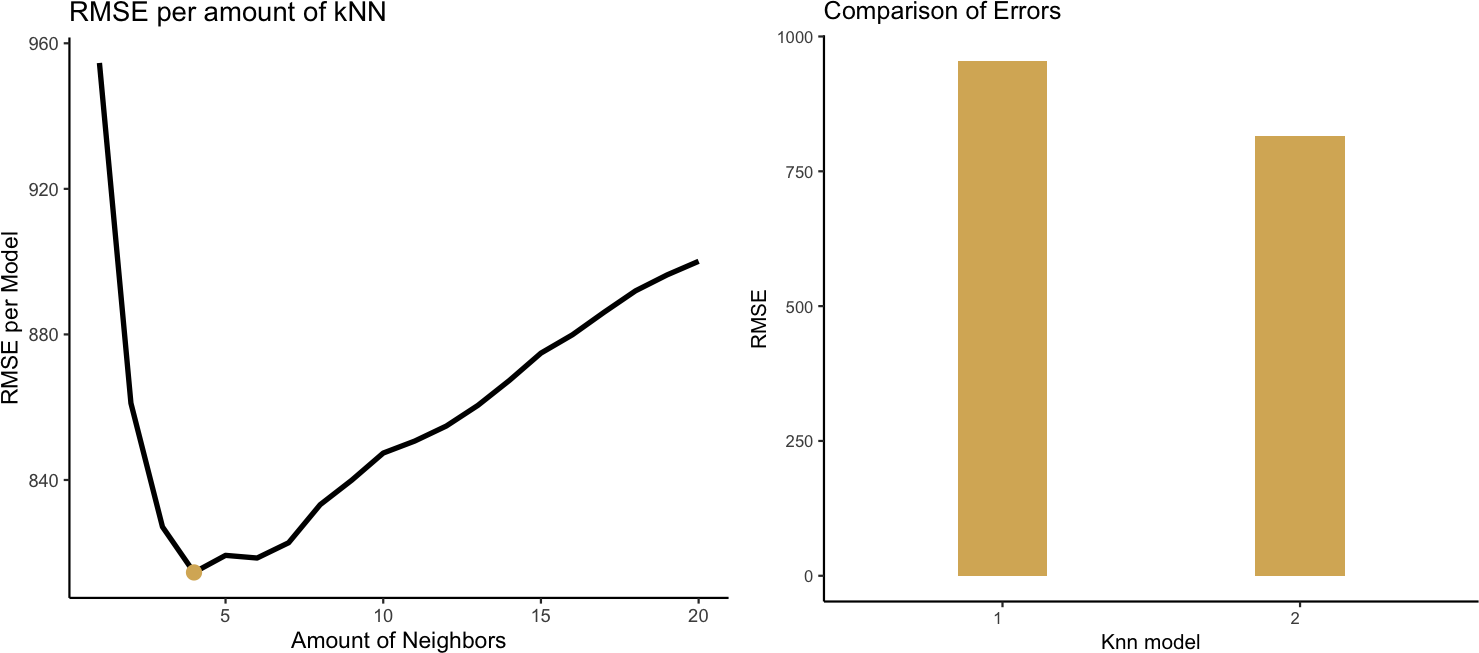
\includegraphics[width=0.5\linewidth,]{Diamonds_PDF_files/figure-latex/knn double plot-1}

}

\caption{Evolution of RMSE with respect to k and difference of RMSE for k = 1 and k = 4}\label{fig:knn double plot}
\end{figure}

As stated earlier, the table above shows how the ME got worse for \(k\)
= 4, but better with RMSE once the model was optimized. In this
analysis, one of the main goals is to reduce the variation between
predicted and real price. Therefore, the difference of \$140.00 is more
important even when the ME slightly increases. Between \(k\) = 1 and
\(k\) = 4 for the \(k\)-NN model, \(k\) = 4 with an RMSE of \$814.60
will predict prices better.

\hypertarget{decision-trees}{%
\subsection{Decision Trees}\label{decision-trees}}

There are four methods within this section that show various ways on how
trees are built. They include a regression tree, boosted tree, bagged
tree, and a random forest. The regression tree is most transparent and
easy to interpret while the other three combine results from multiple
trees.

\hypertarget{regression-tree-overview}{%
\paragraph{Regression Tree Overview}\label{regression-tree-overview}}

A regression tree is a flexible data-driven method that can be used for
prediction of a continuous variable. The tree separates `records into
subgroups by creating splits on predictors. These splits create logical
rules that are homogeneous.' Those splits `divide the data into subsets,
that is, branches, nodes, and leaves. Like decision trees, regression
trees select splits that decrease the dispersion of target attribute
values. Thus, the target attribute values can be predicted from their
mean values in the leaves' which reduces the variance of the target
variable.

\hypertarget{model-structure-and-analysis}{%
\paragraph{Model Structure and
Analysis}\label{model-structure-and-analysis}}

Since the tree proactively takes into consideration the most important
attributes to split on, multiple trees are created to check its
validity. This idea stemmed from wanting to ensure that by removing
variables due to their weak relationship to the predictor variable or by
pruning, the results produced the best ME and RMSE. Within the three
regression models, all have the same error rates. In addition, there are
eight terminal nodes for each model and all had \texttt{width},
\texttt{length}, \texttt{carat}, and \texttt{depth} being the most
important features to predict \texttt{price}. To exemplify this, we show
the original regression tree that first splits on \texttt{width}
\textless{} 6.33, seven splits total and uses the following for the
primary splits: \texttt{width} \textless{} 6.325, \texttt{carat}
\textless{} 0.985, \texttt{length} \textless{} 6.325 and \texttt{depth}
\textless{} 3.935.

\begin{figure}[H]

{\centering 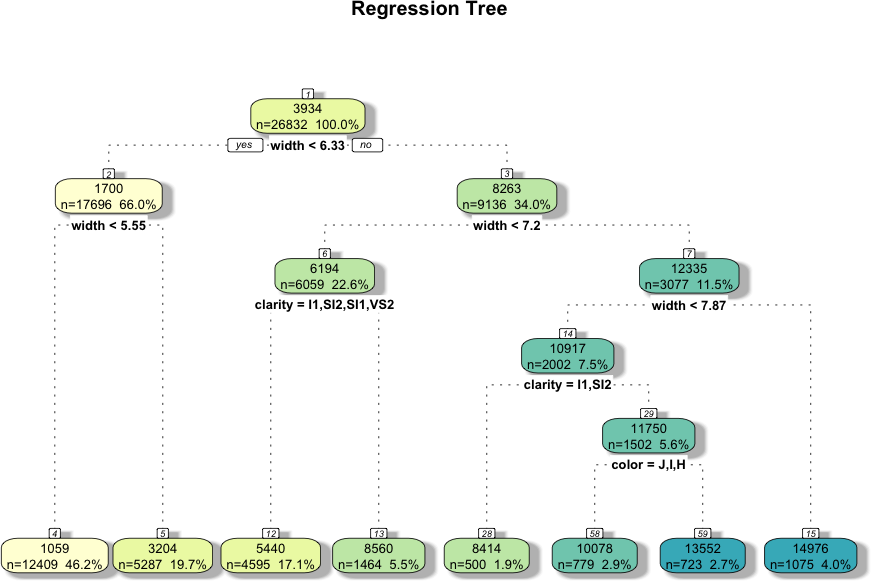
\includegraphics[width=\linewidth,]{Diamonds_PDF_files/figure-latex/Default Regression Tree-1}

}

\caption{Regression tree diagram}\label{fig:Default Regression Tree}
\end{figure}

\hypertarget{boosted-tree}{%
\subsubsection{Boosted Tree}\label{boosted-tree}}

\hypertarget{overview-1}{%
\paragraph{Overview}\label{overview-1}}

Boosted trees are a type of ensemble model that `transforms weak
decision trees into strong learners. Each new tree is built considering
the errors of previous trees.' The idea behind boosting is to train a
series of weak models additively, with each model attempting to correct
the errors made by the previous model. Since this model is prone to
overfitting, the parameters need to be carefully considered so that the
lowest error rates can be achieved.

\hypertarget{model-structure-and-analysis-1}{%
\paragraph{Model Structure and
Analysis}\label{model-structure-and-analysis-1}}

There is a wide variety of parameters that can be chosen for a boosted
tree. Therefore, those options were used differently to choose the best
model based off the number of predictors and how deep each tree would be
allowed to interact. The main difference between each model is the
number of trees ran. As the size of the tree increases, the better the
model because it only considered the most important factors.

The best boosted model was the one with 100 trees and three
cross-validation folds. The tree used six predictors to produce a model
with a ME of \$9.00 and RMSE of \$1,170.30. What is fascinating about
this tree comes from the importance variables chart. In the regression
tree, \texttt{clarity} was one of the three least important factors, but
here we see that it as the fourth which is above \texttt{length}.

\hypertarget{bagged-tree}{%
\subsubsection{Bagged Tree}\label{bagged-tree}}

\hypertarget{overview-2}{%
\paragraph{Overview}\label{overview-2}}

The third method is bagged trees. This type of model `combines the
predictions from multiple machine learning algorithms together to make
more accurate predictions than any individual model.' The objective with
bagging is to train a large number of decision trees on different
subsets of the training data, and then average the predictions of all
the trees to make a final prediction. This model has the ability to
reduce variance because it introduces randomness into the training
process.

\hypertarget{model-structure-and-analysis-2}{%
\paragraph{Model Structure and
Analysis}\label{model-structure-and-analysis-2}}

This model is pretty straight forward because the best model was built
by sticking with the basics. `The only parameters when bagging decision
trees is the number of samples and hence the number of trees to include.
This can be chosen by increasing the number of trees on run after run
until the accuracy begins to stop showing improvement.' Overall, the
bagging tree predicts \texttt{price} better than the regression tree,
but worse than boosting. The ME was the lowest at \$0.93, but what is
more important to consider is the RMSE which is \$1,248.77.

\hypertarget{random-forest}{%
\subsubsection{Random Forest}\label{random-forest}}

\hypertarget{overview-3}{%
\paragraph{Overview}\label{overview-3}}

`Random forests are a special case of bagging, a method for improving
predictive power by combining multiple classifiers or prediction
algorithms.' They are an ensemble based on bagged trees which involves
training each tree on a bootstrapped sample of the original data.

\hypertarget{model-structure-1}{%
\paragraph{Model Structure}\label{model-structure-1}}

Similar to the bagged trees, random forests are pretty simplistic. The
main focus in this section was to check how many trees should be run
within the model. There is a trade-off between computational power and
RMSE. For example, what is the difference in RMSE if the model was built
off of 100 trees versus 60? The model with 100 trees was the best model
with an RMSE of \$575.42.

\begin{figure}[H]

{\centering 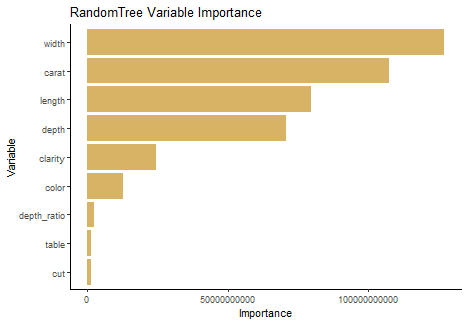
\includegraphics[width=0.5\linewidth,]{Diamonds_PDF_files/figure-latex/RF Variable Importance-1}

}

\caption{Variable importance for random forest}\label{fig:RF Variable Importance}
\end{figure}

Throughout this entire section, typically the lower RMSE produced the
best model. Additionally up to this point, there have been three or four
variables that were most importance to the model. In the random forest
though, there is much more weight on features such as \texttt{clarity}
and \texttt{color}. In random forests, we proposed a trade-off with
picking a model with less trees because an analyst would want to choose
the parsimonious model. Therefore, the random forest with 60 trees had a
slightly higher RMSE at a difference of approximately \$2 which gave a
\$577.63 for the RMSE.

\hypertarget{decision-tree-summary-table}{%
\subsubsection{Decision Tree Summary
Table}\label{decision-tree-summary-table}}

\begin{table}[!h]

\caption{\label{tab:RegTree Summary}Accuracy measures of decision tree models}
\centering
\begin{tabu} to \linewidth {>{\raggedright}X>{\raggedright}X>{\raggedright}X>{\raggedright}X>{\raggedright}X>{\raggedright}X}
\hline
  & ME & RMSE & MAE & MPE & MAPE\\
\hline
Reg. Tree & 6.1 & 1267.15 & 846.93 & -14.54 & 33.08\\
\hline
Exclus. RT & 6.1 & 1267.15 & 846.93 & -14.54 & 33.08\\
\hline
Pruned RT & 6.1 & 1267.15 & 846.93 & -14.54 & 33.08\\
\hline
Boost10 & -3.9 & 3660.42 & 2765.96 & -144.49 & 171.65\\
\hline
Boost30 & 2.54 & 1531.52 & 985.7 & -35.26 & 46.86\\
\hline
Boost100 & 9 & 1170.3 & 680.22 & -12.85 & 26.22\\
\hline
Bagging & 0.93 & 1248.77 & 808.93 & -14.35 & 31.45\\
\hline
RndmFrst & 2.97 & 577.63 & 289.51 & -1.4 & 7.24\\
\hline
\end{tabu}
\end{table}

\begin{figure}[H]

{\centering 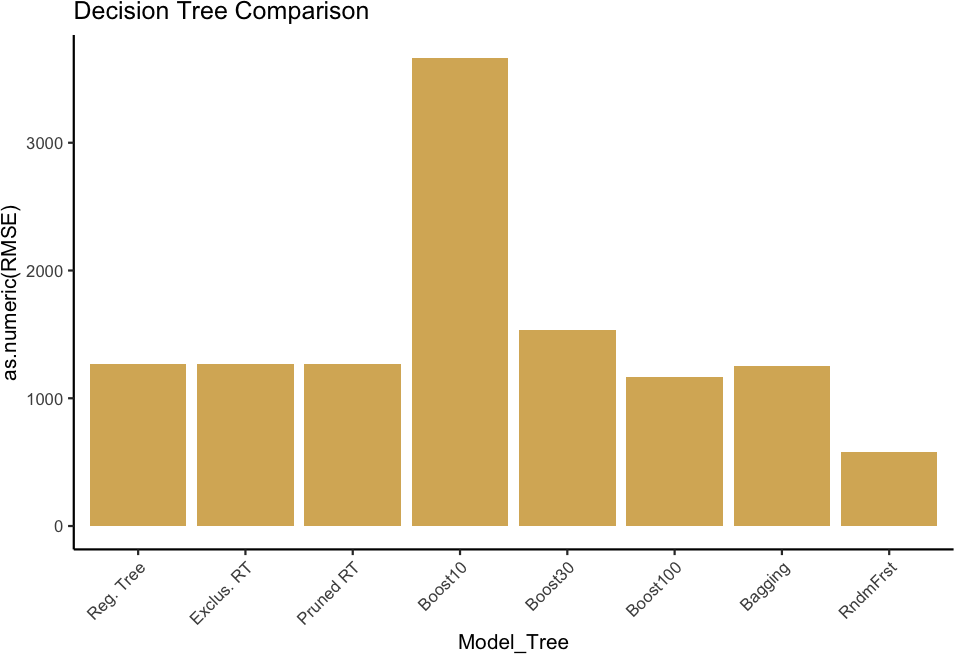
\includegraphics[width=0.5\linewidth,]{Diamonds_PDF_files/figure-latex/RegTree Summary-1}

}

\caption{RMSE of decision trees}\label{fig:RegTree Summary}
\end{figure}

Throughout the four methods mentioned, the random forest model proved to
be the most effective in predicting \texttt{price} with a RMSE of
\$577.63, which is more than two times smaller than the best boosting
model. Although not all of the models results are shown, a breakdown of
their error results can be seen within the table above. Overall, the
regression tree, bagging and boosting were all within \$100 RMSE
difference, but no match for the random forest.

\hypertarget{neuralnetworks}{%
\subsection{NeuralNetworks}\label{neuralnetworks}}

\hypertarget{basic-concept}{%
\subsubsection{Basic Concept}\label{basic-concept}}

Artificial neural networks are a method of machine learning that
receives the name due to a comparison made with actual neurons in the
human brain. They consist various nodes that communicate with each other
to predict an outcome based on the relationships that were determined in
the process. Neural nets have proven to be very good at predicting
values, through regression or classification and have been the center of
much research in the past years. Though this method was once considered
un useful, with the improvement of computational power, it has acquired
new popularity for prediction of images, speech recognition and
non-explicit trends. (Hardesty, 2017)

The basic parts of a neural networks are: the structure, composed of
layers and nodes, the weights, and the activation function. The first
consists of the different components used to train a neural network, ie
the explanatory variables and their connection. These independent
variables are considered the \emph{input nodes} and the outcome variable
the \emph{output node}. The layers in between these to are called the
\emph{hidden layers} as these are used to calculate the output but have
no easily association of there value with regards to the outcome. This
is why neural networks are considered by some like a \textbf{black box},
where the exact method for predicting is not easily explained to those
who are not well informed. The weights are used to pass a certain amount
of a value to the next node which after passing through the activation
function will pass on to the next, and so on. This weighting can be
assigned randomly or by specific methods, depending on the problem at
hand and analyst discretion. Similarly, the activation function
calculates the position in a curve, ie the expected value of the
prediction. This as well changes per prediction problem and analyst
discretion. While some are considered better for certain tasks there is
no limiting factor in the way a neural net is structured.

\hypertarget{data-preprocessing}{%
\subsubsection{Data preprocessing}\label{data-preprocessing}}

Due to the fact that in every node we calculate the position of the
prediction in a curve, the scale of the values used affects the output
of every node. Moreover, since we use all types of variables for
prediction in neural networks (continuous and categorical) the
difference in amplitude is very important. This is why it is standard
procedure to normalize the data so they are all in the same scale.

\hypertarget{model-structures}{%
\subsubsection{Model Structures}\label{model-structures}}

There is no standard or ideal way of setting up the amount of layers in
a network, but common rule of thumb is to start with the same amount of
input variables and then reduce to see if this improves. (Shmueli, et
al.~2018: 286) In this case, it was decided to follow the following
structures:

\begin{itemize}
\item
  The first model is composed of all the variables (26 explanatory) and
  a single hidden layer of one node. All models have only one output
  node as the desired outcome is a single prediction of price. This
  model is considered to be the most basic and should in theory have the
  least predictive performance.
\item
  The second model includes a hidden layer of 26 nodes, so it equals the
  input nodes.
\item
  To see if there is an improvement, we do another model with just 13
  nodes in a single hidden layer.
\end{itemize}

Of these single layer models, the best is the one with 26 nodes. We
measure this by looking at the error in prediction, also called the
accuracy. There are many ways of measuring this, but as mentioned
before, the two we looked at are the Mean Error, as a measure of
accuracy, and Root Mean Squared Error, as a measure of precision. For
the 26 node model, the RMSE is \$745.16 vs \$744.04 for the 13 node net.
While just looking at this configuration one could infer using less
nodes is better, after multiple tests it is concluded that keeping the
26 nodes as the first hidden layer is best for reducing the RMSE going
forward.

The next configuration tested is adding 2 additional hidden layers, one
of 26 additional nodes, and another of 13. Just by using this
configuration, the model RMSE reduced to \$627.65. As this is already a
rather low RMSE, in comparison to previous neural networks, as well as
other models seen above, it was decided to keep this structure as the
definitive one for establishing the most accurate prediction.

The next two adjustments made are regarding the weights and the
activation function. This structure was adjusted to use the
``\emph{Glorot Normal}'' weight initiation method. This initiation
method consists of assigning weights to the nodes using a de probability
curve of a truncated normal distribution as so:

\textbf{Glorot Normal Initialization:}

\[w_{i} \sim Gaussian \left(\mu = 0, \sigma^{2} = \sqrt{\frac{2} {u_{in} + u_{out} }}\right)\]

where:

\(u_{in}\) = number of input nodes

\(u_{out}\) = number of output nodes

This initiation method demonstrated much better results than others such
as the normal distribution, uniform distribution of the Glorot Uniform,
which is why we kept it for the final model.

Finally regarding the activation function, many options are available as
well. Depending on the problem at hand, one can use different functions
that draw different curves and hence produce different predictions. The
one used for our case was a \emph{sigmoid} activation which by different
literature is the most commonly used due to its good performance
results. Though we tested others like \emph{``relu''} or
\emph{``softplus''}, sigmoid ended being the most accurate predicting.

\hypertarget{neural-net-summary-table}{%
\subsubsection{Neural Net Summary
Table}\label{neural-net-summary-table}}

\begin{table}[!h]

\caption{\label{tab:NN Summary}Accuracy measures of neural network models}
\centering
\begin{tabu} to \linewidth {>{\raggedright}X>{\raggedright}X>{\raggedright}X>{\raggedright}X>{\raggedright}X>{\raggedright}X}
\hline
  & ME & RMSE & MAE & MPE & MAPE\\
\hline
L1 N1 & -246.53 & 1175.41 & 890.47 & -53.75 & 63.14\\
\hline
L1 N26 & -88.66 & 760.74 & 465.61 & -11.44 & 18.28\\
\hline
L1 N13 & -90.67 & 749.84 & 452.97 & -11.41 & 17.76\\
\hline
L2 N26 & 22.48 & 636.79 & 364.38 & -4.75 & 12.82\\
\hline
L2 N26 G & -45.24 & 662.5 & 383.93 & -8.36 & 14.19\\
\hline
L2 N26 G LR & -51.05 & 591.6 & 340.12 & -5.26 & 11.16\\
\hline
\end{tabu}
\end{table}

\begin{figure}[H]

{\centering 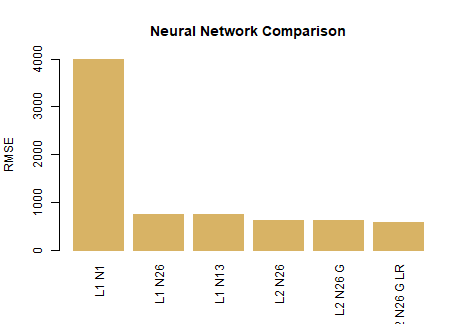
\includegraphics[width=0.5\linewidth,]{Diamonds_PDF_files/figure-latex/NN Summary-1}

}

\caption{RMSE of neural networks}\label{fig:NN Summary}
\end{figure}

As can be seen, the predictive performance of the neural networks can
vary a lot depending on the structure and parameters chosen. The
negative point in this method is the requirement of human input to
adjust the model to learn more precisely. Nevertheless, once the many
trials have been executed, the results are very positive for a good
predictive model.

\begin{figure}
\centering
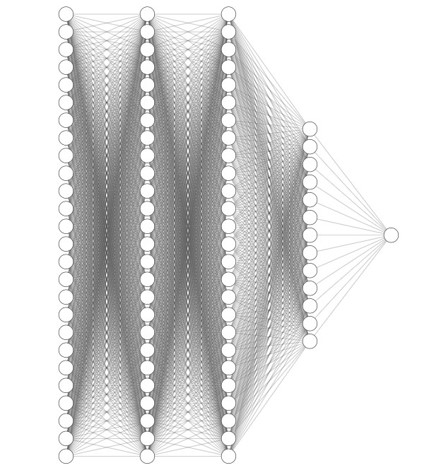
\includegraphics{NN_res.jpeg}
\caption{Visual description of Neural Network}
\end{figure}

\hypertarget{ensembles}{%
\subsection{Ensembles}\label{ensembles}}

\hypertarget{overview-model-structure-and-analysis}{%
\paragraph{Overview, Model Structure and
Analysis}\label{overview-model-structure-and-analysis}}

`Ensemble methods is a machine learning technique that combines several
base models in order to produce one optimal predictive model.' The
simplest approach is to combine predictions from each method above that
had the best/lowest RMSE. To accurately compare models, the mean is
taken over the four models to compute the average predicted
\texttt{price} and find the error rates between the calculated
\texttt{price} and real prices. As the table reveals, the RMSE is
\$588.34 which is pretty close to random forests and the best neural
network in terms of variance.

\begin{table}[!h]

\caption{\label{tab:ensemble error table}Accuracy measures of five main models}
\centering
\begin{tabu} to \linewidth {>{\raggedright}X>{\raggedright}X>{\raggedright}X>{\raggedright}X>{\raggedright}X>{\raggedright}X}
\hline
  & ME & RMSE & MAE & MPE & MAPE\\
\hline
Multiple Linear Regression & 50.4 & 810.16 & 405.06 & -0.84 & 10.4\\
\hline
Random Forest & 2.97 & 577.63 & 289.51 & -1.4 & 7.24\\
\hline
k-Nearest Neighbor & 40.86 & 814.59 & 431.29 & -2.45 & 12.14\\
\hline
Neural Network & -51.05 & 591.6 & 340.12 & -5.26 & 11.16\\
\hline
Ensemble & 10.8 & 583.21 & 308.04 & -2.49 & 8.67\\
\hline
\end{tabu}
\end{table}

\hypertarget{conclusion}{%
\section{Conclusion}\label{conclusion}}

After reviewing the results and performance of each model in the
previous section, we can conclude that the best models are the Random
Forest and Neural Network. This is because they have the lowest error
measures that we take into consideration throughout this analysis. In
addition, more can be deducted by looking at the errors plotted in a
graph.

\hypertarget{plots-of-predicted-price}{%
\subsection{Plots of Predicted Price}\label{plots-of-predicted-price}}

We can see how the predicted diamond price behaves with respect to the
real price by utilizing each of the methods and mapping the three
categorical variables. This recognizes the models' respective precision.
When there are more observations closer to the diagonal line, the
precision is higher. Within the scatter plots, the Random Forest and the
Neural Network are more condensed. On the other hand, \(k\)-NN and MLR
are more sparse. A similar situation happens when adding each of the
categorical values as a color differentiator.

\hypertarget{predicted-price-vs-real-price-by-clarity}{%
\subsubsection{Predicted Price vs Real Price by
Clarity}\label{predicted-price-vs-real-price-by-clarity}}

The multiple linear regression seems to have more issues predicting
price of diamonds with better \texttt{clarity} in the mid to high priced
diamonds. However, there is generally no clear discernible pattern per
\texttt{clarity}. The abundance of the browner colored points is due to
the existence of mid to low level clarities in the data set.

\begin{figure}[H]

{\centering 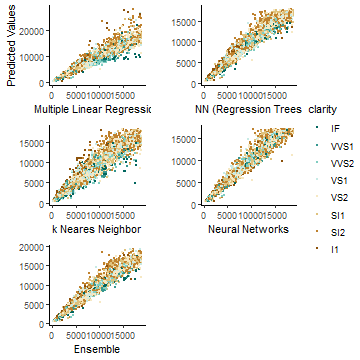
\includegraphics[width=\linewidth,]{Diamonds_PDF_files/figure-latex/Ensemble Summary Plot-1}

}

\caption{Predicted Price vs Real Price by Clarity}\label{fig:Ensemble Summary Plot}
\end{figure}

\newpage

\hypertarget{predicted-price-vs-real-price-by-color}{%
\subsubsection{Predicted Price vs Real Price by
Color}\label{predicted-price-vs-real-price-by-color}}

With regards to \texttt{color}, we see more of the more teal-colored
points. However, there is still no pattern that indicates better or
worse performance per \texttt{color} type.

\begin{figure}[H]

{\centering 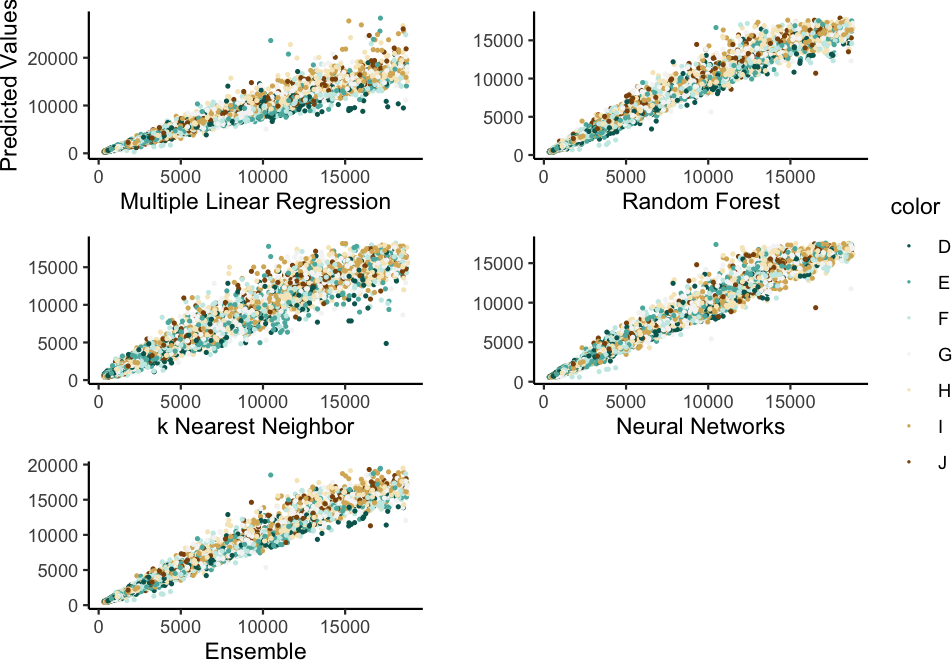
\includegraphics[width=\linewidth,]{Diamonds_PDF_files/figure-latex/Summ Color Plots-1}

}

\caption{Predicted Price vs Real Price by Color}\label{fig:Summ Color Plots}
\end{figure}

\newpage

\hypertarget{predicted-price-vs-real-price-by-cut}{%
\subsubsection{Predicted Price vs Real Price by
Cut}\label{predicted-price-vs-real-price-by-cut}}

Finally, the \texttt{cut} variable shows more \texttt{Ideal} and
\texttt{Premium} cuts. Following the same trend as \texttt{clarity} and
\texttt{color}, there is no pattern for the particular variable.

\begin{figure}[H]

{\centering 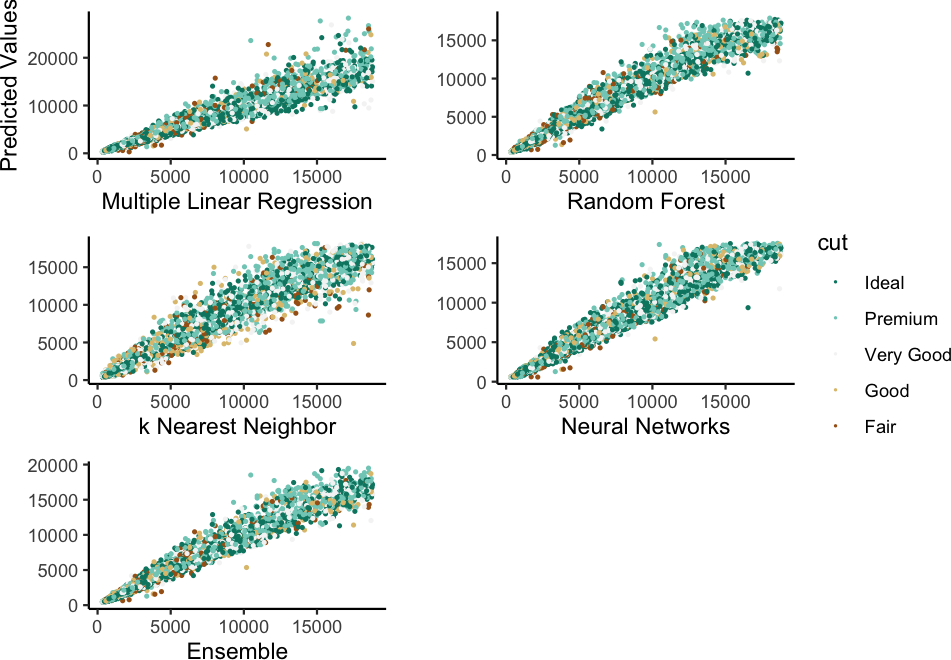
\includegraphics[width=\linewidth,]{Diamonds_PDF_files/figure-latex/Summ Cut Plots-1}

}

\caption{Predicted Price vs Real Price by Cut}\label{fig:Summ Cut Plots}
\end{figure}

The previous graphs show no discernible pattern regarding the
categorical variables. Therefore, the performance of the Random Forest
and the Neural Network is evident with smaller dispersion of the points.
As the difference in error is quite close between these two models, our
final model decision comes down to a matter of analyst preference or
computational power available. We consider, however, that due to the
smaller ME, our recommendation is to use the Random Forest for
predicting diamond prices.

\newpage

\hypertarget{references}{%
\section{References}\label{references}}

Shmueli et al.~(2018). \emph{Data Mining for Business Analytics}. Wiley.

Hardesty, Larry. (2017). {[}Explained: Neural Networks{]} MIT News.
(\url{https://news.mit.edu/2017/explained-neural-networks-deep-learning-0414})

EDA

\begin{itemize}
\tightlist
\item
  \url{https://r-graph-gallery.com/199-correlation-matrix-with-ggally.html}
\item
  \url{http://www.sthda.com/english/wiki/ggplot2-quick-correlation-matrix-heatmap-r-software-and-data-visualization}
\end{itemize}

k-NN

\begin{itemize}
\tightlist
\item
  \url{https://online.stat.psu.edu/stat508/lesson/k\#}:\textasciitilde:text=The\%20larger\%20k\%20is\%2C\%20the,Nearest\%20Neighbors\%20are\%20shown\%20below.
\item
  \url{https://www.analyticsvidhya.com/blog/2018/03/introduction-k-neighbours-algorithm-clustering/}
\end{itemize}

Regression Tree

\begin{itemize}
\tightlist
\item
  \url{https://www.ibm.com/docs/en/db2-warehouse?topic=procedures-regression-trees}
\end{itemize}

Boosted Tree

\begin{itemize}
\tightlist
\item
  \url{https://towardsdatascience.com/introduction-to-boosted-trees-2692b6653b53}\strut \\
\item
  \url{https://leonlok.co.uk/blog/decision-trees-random-forests-gradient-boosting-whats-the-difference/}
\end{itemize}

Bagging Tree

\begin{itemize}
\tightlist
\item
  \url{https://machinelearningmastery.com/bagging-and-random-forest-ensemble-algorithms-for-machine-learning/}
\end{itemize}

Ensemble

\begin{itemize}
\tightlist
\item
  \url{https://towardsdatascience.com/ensemble-methods-in-machine-learning-what-are-they-and-why-use-them-68ec3f9fef5f}
\end{itemize}

\end{document}
